%TC:ignore
\documentclass{article}
\usepackage{caption}
\usepackage{xcolor, colortbl}
\definecolor{RED}{HTML}{EB6231}
\definecolor{YELLOW}{HTML}{E29D26}
\definecolor{BLUE}{HTML}{5D80B4}
\definecolor{LIGHTGREY}{gray}{0.9}
\definecolor{BLUELINK}{HTML}{0645AD}
\definecolor{DARKBLUELINK}{HTML}{0B0080}
\definecolor{LIGHTGREEN}{HTML}{6ABD9B}
\definecolor{GREEN}{HTML}{8FB03E}
\definecolor{PURPLE}{HTML}{BE1E2D}
\definecolor{BROWN}{HTML}{A97C50}
\definecolor{PINK}{HTML}{DA1C5C}

\PassOptionsToPackage{hyphens}{url}
\usepackage{hyperref}
% for linking between references, figures, TOC, etc in the pdf document
\hypersetup{colorlinks,
    linkcolor=DARKBLUELINK,
    anchorcolor=DARKBLUELINK,
    citecolor=DARKBLUELINK,
    filecolor=DARKBLUELINK,
    menucolor=DARKBLUELINK,
    urlcolor=BLUELINK
} % Color citation links in purple
\PassOptionsToPackage{unicode}{hyperref}
\PassOptionsToPackage{naturalnames}{hyperref}

\usepackage[backend=biber,eprint=false,isbn=false,url=false,intitle=true,style=nature,date=year]{biblatex}
\addbibresource{references.bib}

\usepackage[margin=50pt]{geometry}
\usepackage{amssymb,amsfonts,amsmath,amsthm,mathtools}
\usepackage{lmodern}
\usepackage{bm,bbold,bbm}
\usepackage{verbatim}
\usepackage{float}
\usepackage{listings, enumerate, enumitem}
\usepackage{pgfplots, pgf,tikz}
\usepgfplotslibrary{fillbetween}

\pgfplotsset{every axis/.append style={line width=1pt}}
\pgfplotscreateplotcyclelist{colors}{LIGHTGREEN\\YELLOW\\RED\\GREEN\\BLUE\\}


\pdfinclusioncopyfonts=1

\renewcommand{\baselinestretch}{1.5}
\renewcommand{\arraystretch}{0.6}
\frenchspacing

\renewcommand{\thetable}{S\arabic{table}}
\renewcommand{\thefigure}{S\arabic{figure}}
\renewcommand{\theequation}{S.\arabic{equation}}

\newcommand{\UniDimArray}[1]{\bm{#1}}
\newcommand{\BiDimArray}[1]{\bm{#1}}
\newcommand{\der}{\text{d}}
\newcommand{\e}{\text{e}}
\newcommand{\Ne}{N_{\text{e}}}

% Genotype-Phenotype-Fitness
\newcommand{\NbrSites}{n}
\newcommand{\Geno}{\mathbb{G}}
\newcommand{\GenoDer}{\Geno^{\prime}}
\newcommand{\Neighbors}{\mathcal{M}}
\newcommand{\setNeighbors}{\Neighbors\left(\Geno\right)}
\newcommand{\Observed}{\mathcal{O}}
\newcommand{\PhenoDef}{x}
\newcommand{\PhenoParam}{\lambda}
\newcommand{\PhenoParamSet}{\Lambda}
\newcommand{\GenoPhenoMap}{H_{\PhenoParam}}
\newcommand{\Pheno}{\GenoPhenoMap\left(\Geno\right)}
\newcommand{\PhenoDer}{\GenoPhenoMap\left(\GenoDer\right)}
\newcommand{\FitParam}{\theta}
\newcommand{\FitParamSet}{\Theta}
\newcommand{\PhenoFitMapDef}{F}
\newcommand{\PhenoFitMap}{\PhenoFitMapDef_{\FitParam}}
\newcommand{\FitDef}{y}
\newcommand{\Fit}{\PhenoFitMap\left(\Pheno\right)}
\newcommand{\FitDer}{\PhenoFitMap\left(\PhenoDer\right)}
\newcommand{\Pfix}{P}
\newcommand{\SelCoeff}{S_{\PhenoParam, \FitParam}}
\newcommand{\Normalize}{\mathcal{Z}_{\PhenoParam, \FitParam}}

\begin{document}
    \part*{Supplementary materials}
    \tableofcontents
    \newpage


    \section{General formalism}\label{sec:general-formalism}

    \subsection{Genotype to phenotype map}\label{subsec:genotype-to-phenotype-map}
    DNA sequence evolution is modelled under an origin-fixation model~\cite{mccandlish_modeling_2014}, meaning that the whole population is considered monomorphic and only the succession of fixation events are modeled.
    We consider the reconstructed ancestral DNA sequence as the reference sequence, and we model the evolution of the DNA sequence by substitutions of one nucleotide at a time occurring along the branch leading to the derived sequence.
    \begin{center}
        \captionof{figure}{Example of substitutions}
        \includegraphics[width=0.6\linewidth, page=1]{substitutions.pdf}
        \label{fig:substitutions}
    \end{center}

    A genotype, $\Geno$, is a DNA sequence of $\NbrSites$ nucleotide sites:
    \begin{align}
        \Geno \in \left\{ A, C, G, T \right\}^{\NbrSites}.
    \end{align}

    In the example of figure~\ref{fig:substitutions}, the reference genotype is:
    \begin{align*}
        \Geno = \text{ATCGATGCTTCG}.
    \end{align*}

    The phenotype, $\PhenoDef$, is assumed to be a continuous variable between $0$ and $1$, with the boundaries corresponding to the extreme phenotypes, while 0.5 corresponds to the reference phenotype:
    \begin{align}
        \PhenoDef \in \left[ 0, 1 \right].
    \end{align}

    And the genotype to phenotype map, $\GenoPhenoMap$, is a function of the genotype and a set of parameters $\PhenoParam \in \PhenoParamSet$:
    \begin{align}
        \GenoPhenoMap : & \left\{ A, C, G, T \right\}^{\NbrSites} \to \left[ 0, 1 \right], \\
        & \Geno \mapsto \PhenoDef.
    \end{align}
    In the example of figure~\ref{fig:substitutions}, the phenotypes corresponding to ancestral sequences and the sequence after a substitution should be a real number between $0$ and $1$, such as for example:
    \begin{align*}
        \begin{dcases}
            \GenoPhenoMap (\text{ATCGAT\textbf{G}C\textbf{T}TCG} ) & = 0.5. \\
            \GenoPhenoMap (\text{ATCGAT{\color{BLUE}{\textbf{C}}}C\textbf{T}TCG} ) & = 0.813. \\
            \GenoPhenoMap (\text{ATCGAT\textbf{G}C{\color{LIGHTGREEN}{\textbf{A}}}TCG} ) & = 0.752.
        \end{dcases}
    \end{align*}

    In the following the genotype to phenotype map is assumed to be known, meaning that the phenotype is a deterministic function of the genotype and that the parameters $\PhenoParam$ are fixed.
    This representation is a general case, and we apply it to the binding affinity in two different ways in the following sections.

    \subsection{Phenotype to fitness map}\label{subsec:phenotype-to-fitness-map}
    The fitness, $\FitDef$, is a positive real number giving the relative reproductive success.
    The phenotype to fitness map, $\PhenoFitMap$, is a function of the phenotype ($\PhenoDef$) and a set of parameters $\FitParam \in \FitParamSet$:
    \begin{align}
        \PhenoFitMap : & \left[ 0, 1 \right] \to \mathbb{R}_{+}, \\
        & \PhenoDef \mapsto \FitDef.
    \end{align}
    In this case, the phenotype to fitness map is not assumed to be known.
    Instead, we restrict the set of possible fitness functions to a set of parametric functions representing different selection regimes: neutral, stabilizing selection and directional selection.
    In this different selection regimes, the fitness function is defined on a different set of parameters $\FitParam \in \FitParamSet$ that are specific to each selection regime and of different dimensionality.

    \subsubsection{Neutral model}
    In the neutral model, all phenotypes have the same fitness.
    \begin{align}
        \PhenoFitMapDef (\PhenoDef) = 1.
    \end{align}
    In such a case, the fitness function is constant and the set of parameters is empty:
    \begin{gather}
        \FitParamSet = \emptyset.
    \end{gather}

    \subsubsection{Stabilizing selection}
    In the stabilizing selection model, the fitness is maximal at the intermediate phenotype (0.5), and decreases as the phenotype moves away from the optimum.
    We used a Beta distribution to model the fitness function:
    \begin{align}
        \PhenoFitMapDef_{\alpha} (\PhenoDef) = \frac {\Gamma (2 \alpha )}{\Gamma (\alpha )^2} \PhenoDef^{\alpha -1}(1-\PhenoDef)^{\alpha -1},
    \end{align}
    where $\Gamma$ is the gamma function:
    \begin{align}
        \Gamma (z)=\int _{0}^{\infty }t^{z-1}e^{-t} \der t.
    \end{align}

    In this case, the fitness function is parameterized by a single parameter $\alpha$ and the parameter space is thus 1-dimensional:
    \begin{gather}
        \begin{cases}
            \FitParam = \alpha,\\
            \FitParamSet = \mathbb{R}_{+}.
        \end{cases}
    \end{gather}
    Importantly, the case $\alpha = 1$ corresponds to the neutral model, such that the two models are nested.

    \subsubsection{Directional selection}
    In the directional selection model, the fitness is maximal at one of the extreme phenotypes and minimal at the other extreme.
    We used a Beta function to model the fitness function:
    \begin{align}
        \PhenoFitMapDef_{\alpha, \beta} (\PhenoDef) = \frac {\Gamma (\alpha +\beta )}{\Gamma (\alpha )\Gamma (\beta )} \PhenoDef^{\alpha -1}(1-\PhenoDef)^{\beta -1},
    \end{align}
    where $\Gamma$ is the gamma function:
    \begin{align}
        \Gamma (z)=\int _{0}^{\infty }t^{z-1}e^{-t} \der t.
    \end{align}

    In this case, the fitness function is parameterized by two parameters $\FitParam$ and the parameter space is 2-dimensional:
    \begin{gather}
        \begin{cases}
            \FitParam = (\alpha, \beta),\\
            \FitParamSet = \mathbb{R}_{+} \times \mathbb{R}_{+}.
        \end{cases}
    \end{gather}

    Importantly, the case where $\alpha = \beta $ corresponds to the stabilizing selection model, such that the two models are nested.
    Because the neutral model is nested in the stabilizing selection model, and the stabilizing selection model is nested in the directional selection model, the three models are nested.

    \begin{center}
        \captionof{figure}{Phenotype to fitness map ($\PhenoFitMap$)}
        \begin{tikzpicture}
            \begin{axis}
                [
                width=0.6\textwidth,
                height=0.5\textwidth,
                cycle list name=colors,
                domain=0:1,
                samples=100,
                xlabel={Phenotype ($\PhenoDef$)},
                ylabel={Fitness ($\FitDef = \PhenoFitMap(\PhenoDef)$)},
                ymin=0.0, ymax=5.0,
                legend entries={Neutral,Stabilizing selection ($\PhenoFitMapDef_{2}$),Stabilizing selection ($\PhenoFitMapDef_{8}$), Directional selection ($\PhenoFitMapDef_{1, 5}$), Directional selection ($\PhenoFitMapDef_{5, 1}$)},
                legend cell align=left,
                minor tick num=2,
                axis x line=bottom,
                axis y line=left,
                legend style={at={(0.2,0.99)},anchor=north west}
                ]
                % Beta(1,1): Normalization constant is 1
                \addplot[thick, YELLOW] {1.0};
                % Beta(2,2): Normalization constant is 6
                \addplot[thick, GREEN] {6*x^(2-1)*(1-x)^(2-1)};
                % Beta(8,8): Normalization constant is 51480
                \addplot[thick, LIGHTGREEN] {51480*x^(8-1)*(1-x)^(8-1)};
                % Beta(1,5): Normalization constant is 5
                \addplot[thick, RED] {5*x^(1-1)*(1-x)^(5-1)};
                % Beta(5,1): Normalization constant is 5
                \addplot[thick, BLUE] {5*x^(5-1)*(1-x)^(1-1)};
            \end{axis}
        \end{tikzpicture}
        \label{fig:phenotype-to-fitness-map}
    \end{center}

    \newpage

    \subsection{Genotype to fitness map}\label{subsec:genotype-to-fitness-map}

    To summarize, the genotype ($\Geno$) is first mapped to a phenotype ($\PhenoDef$) using the genotype to phenotype map ($\GenoPhenoMap$).
    Then the phenotype is mapped to a fitness ($\FitDef$) using the phenotype to fitness map ($\PhenoFitMap$).
    Altogether, the genotype to fitness map is given by the composition of the two maps:
    \begin{align}
        \Geno \xmapsto{\GenoPhenoMap} \PhenoDef \xmapsto{\PhenoFitMap} \FitDef.
    \end{align}
    The genotype to phenotype map ($\GenoPhenoMap$) is assumed to be known, while the phenotype to fitness map ($\PhenoFitMap$) is assumed to be unknown and restricted to a set of parametric functions representing different selection regimes.

    \subsection{Probability of fixation}\label{subsec:probability-of-fixation}

    Given the currently fixed sequence $\Geno$, we define $\setNeighbors$ as the set of all possible mutant that are one nucleotide away from $\Geno$.
    For a sequence of $\NbrSites$ nucleotide sites, $\left| \setNeighbors \right| = 3 \NbrSites$, since each site has $3$ possible mutations.
    For each mutant sequence $\GenoDer \in \setNeighbors$, we can compute its fitness $\FitDer$.

    In the example of figure~\ref{fig:substitutions}, the set of neighbors of the sequence $\Geno$ is:
    \begin{align*}
        \Geno = \hspace{0.75em} & \text{ATCGATGCTTCG} \\
        \text{and } \setNeighbors = \{ & \text{\textbf{C}TCGATGCTTCG}, \\
        & \text{\textbf{G}TCGATGCTTCG}, \\
        & \text{\textbf{T}TCGATGCTTCG}, \\
        & \text{A\textbf{A}CGATGCTTCG}, \\
        & \text{A\textbf{C}CGATGCTTCG}, \\
        & \quad \quad \quad \quad \quad \vdots  \\
        & \text{ATCGATGCTTC\textbf{T}} \}
    \end{align*}

    The selection coefficient $\SelCoeff \left( \Geno,\GenoDer\right)$ associated to a change is the difference between the fitness of the derived sequence and the fitness of the reference sequence:
    \begin{align}
        \SelCoeff : & \left\{ A, C, G, T \right\}^{\NbrSites} \times \left\{ A, C, G, T \right\}^{\NbrSites} \to \mathbb{R}, \\
        & \left( \Geno,\GenoDer\right) \mapsto \FitDer - \Fit.
    \end{align}

    Then, the scaled probability of fixation of a mutation, $\Pfix$ is a function of the selection coefficient, defined as:
    \begin{align}
        \Pfix : &  \mathbb{R} \to \mathbb{R}_{+}, \\
        & s \mapsto \dfrac{s}{1 - \e^{-s}}.
    \end{align}

    \newpage
    \begin{center}
        \captionof{figure}{Scaled probability of fixation ($\Pfix$)}
        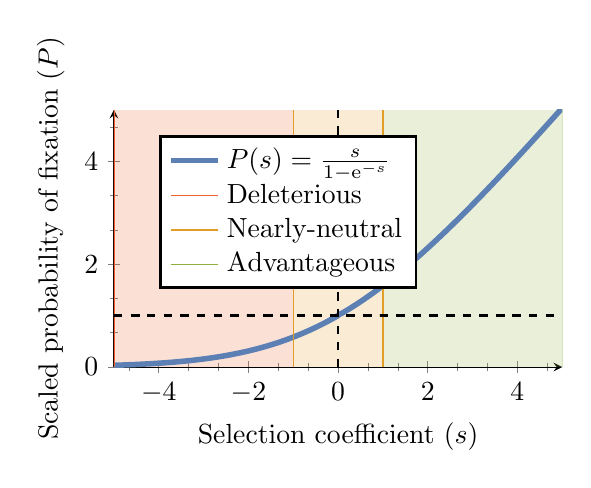
\begin{tikzpicture}
            \begin{axis}
                [
                width=0.6\textwidth,
                height=0.4\textwidth,
                ylabel={Scaled probability of fixation ($\Pfix$)},
                xlabel={Selection coefficient ($s$)},
                domain=-5:5,
                ymin=0.0, ymax=5.0,
                samples=200,
                legend entries={$\Pfix (s) = \frac{s}{1 - \e^{-s}}$,Deleterious,Nearly-neutral,Advantageous},
                legend cell align=left,
                minor tick num=2,
                axis x line=bottom,
                axis y line=left,
                legend style={at={(0.1,0.9)},anchor=north west}
                ]
                \addplot[line width=2.0pt, BLUE]{ x / (1 - exp(- x))};
                \addplot[name path=A, RED, line width=0.5pt] coordinates {(-5, 0) (-5, 5)};
                \addplot[name path=B, YELLOW, line width=0.5pt] coordinates {(-1, 0) (-1, 5)};
                \addplot[name path=D, GREEN, line width=0.5pt] coordinates {(5, 0) (5, 5)};
                \addplot[name path=C, YELLOW, line width=0.5pt] coordinates {(1, 0) (1, 5)};
                \addplot[black, dashed, line width=1.0pt]{1.0};
                \addplot[black, dashed, line width=1.0pt] coordinates {(0, 0) (0, 5)};
                \addplot[fill=RED, opacity=0.2] fill between[ of = A and B];
                \addplot[fill=YELLOW, opacity=0.2] fill between[ of = B and C];
                \addplot[fill=GREEN, opacity=0.2] fill between[ of = C and D];
            \end{axis}
        \end{tikzpicture}
        \label{fig:scaled-probability-of-fixation}
    \end{center}

    Altogether, the scaled probability of fixation from the reference sequence $\Geno$ to a derived sequence $\GenoDer$ is given by:
    \begin{align}
        \Pfix \left( \SelCoeff \left( \Geno,\GenoDer\right)\right).
    \end{align}

    \subsection{Likelihood of the data}\label{subsec:likelihood-of-the-data}
    Now, we consider a set of observed substitutions $\Observed \subset \setNeighbors$ away from the ancestral sequence $\Geno$.
    Importantly, even if several substitutions are observed along the terminal branch, we cannot know the order of the substitutions and the time at which they occurred.
    As such, the substitutions are considered as independent events and thus a sample from the set of all possible substitutions $\setNeighbors$.

    In the example of figure~\ref{fig:substitutions}, the set of observed substitutions $\Observed$ away from the sequence $\Geno$ is:
    \begin{align*}
        \Geno = \hspace{0.75em} & \text{ATCGATGCTTCG} \\
        \text{and } \Observed = \{ & \text{ATCGAT{\color{BLUE}{\textbf{C}}}CTTCG}, \\
        & \text{ATCGATGC{\color{LIGHTGREEN}{\textbf{A}}}TCG} \}
    \end{align*}

    Across all possible mutations ($\GenoDer \in \setNeighbors$), we compute the normalization factor $\Normalize (\Geno)$ as:
    \begin{align}
        \Normalize (\Geno) & = \sum_{\GenoDer \in \setNeighbors} \Pfix \left( \SelCoeff \left( \Geno,\GenoDer\right)\right).
    \end{align}

    Then, from the set of observed substitution $\Observed \subset \setNeighbors$, the likelihood of the data is given by:
    \begin{align}
        \mathcal{L} (\Observed, \Geno | \FitParam, \PhenoParam ) & = \prod_{\GenoDer \in \Observed} \dfrac{\Pfix \left( \SelCoeff \left( \Geno,\GenoDer\right)\right)}{\Normalize (\Geno)}.
    \end{align}

    The parameters $\FitParam$ are estimated by maximizing the likelihood of the data with standard optimization algorithms.

    \newpage

    \section{Application to binding affinity}\label{sec:application-to-binding-affinity}

    For a given DNA sequence, the binding affinity of a transcription factor is obtained via machine learning models.
    The binding affinity is a continuous variable, with high values corresponding to strong binding and low values corresponding to weak binding.
    But, the binding affinity is not constrained to be in the interval $[0, 1]$, hence we need to regularize the binding affinity to be in the unit interval.

    \subsection{Regularization of the phenotype map}\label{subsec:regularization-of-the-phenotype-map}
    The simplest way to regularize the binding affinity is to normalize by the maximum value.

    \subsection{Quantization of the phenotype map}\label{subsec:quantization-of-the-phenotype-map}
    Another way to regularize the binding affinity is to quantize the binding affinity into a discrete number of bins.
    The binding affinity is then mapped to a discrete value corresponding to the bin in which it falls.

    \printbibliography
\end{document}